% LaTeX 简介

考虑到许多网友没有使用过 LaTeX 或者只写过公式, 本文结合小时物理百科做一个简要的介绍.

LaTeX 是一种所见非所得的排版语言, 即用户编辑的是代码, 需要经过编译过程才能获得最终的显示效果. 小时物理百科的 PDF 编译使用 \href{https://www.tug.org/texlive/}{TeXlive}, 而在线编辑器则是我们自行开发的.

一个简单完整的 LaTeX 文档如下(文件名如 \lstinline|test.tex|)\footnote{LaTeX 文档通常使用 UTF-8 编码的文本文档.}
% 未完成:高亮
\begin{lstlisting}
\documentclass{article}
\usepackage{amsmath}

\begin{document}
\title{My Title}
\author{My Name}
\maketitle

\section{Introduction}
Some introduction.

\begin{equation}
a^2 + b^2 = c^2 % is this correct?
\end{equation}

\subsection{Subtitle}
Subsection text.

\end{document}
\end{lstlisting}

编译后效果如\autoref{latxIn_fig1}.
\begin{figure}[ht]
\centering
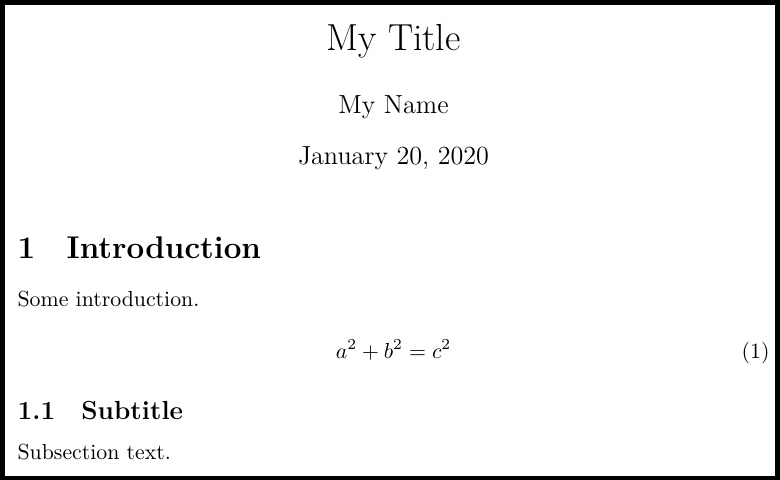
\includegraphics[width=13cm]{./figures/LatxIn1.png}
\caption{排版效果} \label{latxIn_fig1}
\end{figure}
下面我们来解释本例中的代码.

\subsection{环境}
一个完整的 LaTeX 文档是由许多环境构成的, 环境的格式如下
\begin{lstlisting}
\begin{环境名}[可选设置]
...
...
\end{环境名}
\end{lstlisting}
其中 \lstinline|[可选设置]| 通常不需要出现. 在一个完整的 LaTeX 文档中, 最大的环境是 \lstinline|document| 环境(第 4 行), 文档的所有内容(包括其他环境)都在 \lstinline|document| 环境中. 在 \lstinline|document| 环境之前通常会有一些设置, 例如规定文档的类别(第 1 行中的 \lstinline|article|), 使用一些语言拓展包(第 2 行的 \lstinline|amsmath|)等. 这些设置过于复杂, 这里不进行介绍. 一般建议直接直接使用现成的模板.

在 \lstinline|document| 环境中, 我们可以用 \lstinline|\section| 和 \lstinline|\subsection| 等命令把文章划分成不同的章节和子章节. 编译器还可以根据这些命令自动生成目录. 在小时物理百科中, 我们使用四级标题, 分别是 \lstinline|\part|(部分), \lstinline|\section| (词条), \lstinline|\subsection|(节), \lstinline|\subsection|(子节). 注意这些命令只是用于插入对应的标题, 并不构成环境.

另一些常用的环境包括公式环境(第 12 行的 \lstinline|equation|) 和图片环境(未给出).

\subsection{命令}
LaTeX 中命令的格式为反斜杠 \lstinline|\| 加连续的大小写字母. 上面的 \lstinline|\begin{...}| 和 \lstinline|\section| 等都是命令. 有的命令可以单独存在(如第 7 行的 \lstinline|\maketitle|), 而另一些命令需要一个或多个输入, 用花括号表示(如 \lstinline|\begin{...}| 和 \lstinline|\section{...}|).

\subsection{注释}
LaTeX 源码中可以用 \lstinline|% 注释内容| 的格式注释(第 13 行). 注释是给作者看的笔记或批注, 在排版时会被忽略. 如果一行中出现了 \lstinline|%|, 那么这行剩下的内容都会被视为注释. 如果需要插入百分号而不是注释, 使用 \lstinline|\%| 即可.

\subsection{多文件编译}
当文档内容较多时(如一本书), 我们可以将主文件中的内容(比如每节)剪切到一个个独立的文件中, 再通过 \lstinline|\input{文件名}| 命令将这些文档的内容插入主文档中. 例如上面的文档可以划分为两个文件, 主文件 \lstinline|test.tex| 为
\begin{lstlisting}
\documentclass{article}
\usepackage{amsmath}

\begin{document}
\title{My Title}
\author{My Name}
\maketitle

\input{section1.tex}

\end{document}
\end{lstlisting}

子文件 \lstinline|section1.tex| 为
\begin{lstlisting}
\section{Introduction}
Some introduction.

\begin{equation}
a^2 + b^2 = c^2 % is this correct?
\end{equation}

\subsection{Subtitle}
Subsection text.
\end{lstlisting}

在小时物理百科的 LaTeX 模板中, 主文件是 \lstinline|main.tex|, 包含百科所有内容. 每个词条(即 \lstinline|\section|)占一个文件 (如 \lstinline|contents/Sample.tex|), 在编译时会被插入 \lstinline|main.tex|.
